\section{\label{sec:numres}数值结果}

本工作的核心目的，是在单圈微扰论中研究矩阵元 $h_\alpha^{(s)}$，从而把涂抹矩阵元与 $\ms$ 方案中的未涂抹矩阵元联系起来。

一般地，关联两个重正化算符可以用空间动量为零的（无质量）外部夸克态完成，前提是该动量不提供重正化标度（例如在 RI/MOM 方案中）。但为完备起见，我想在微扰论中探索涂抹矩阵元的动量结构。因此，本节简要研究 $h_\alpha^{(s)}$ 中依赖动量的有限部分，它们对上一节的匹配关系并非必需。

\paragraph{解析方法}在给出若干示例结果之前，我简要评论有限外部动量下的计算。引入非零外部动量使计算大为复杂。会出现四个新图，即图 (b)、(c)、(e)、(i)，但单圈水平下图数目的增加并不算繁重。更具挑战性的是动量积分本身。关键困难在于梯度流提供的指数阻尼因子，它阻碍了对积分轻松应用留数定理。此外，这些阻尼因子也使 Feynman 参数的使用复杂化，因为被积函数分母中出现的动量组合一般不是指数的宗量中出现的那些组合，因此无法把被积函数约化为径向对称的形式。指数因子自然地引导人们对图中的传播子引入 Schwinger 表示，但这些一般导致形如
\begin{equation}
\sum_i\int_0^\infty \prod_j\mathrm{d}\alpha^{(j)}\,f^{(i)}\left(\alpha^{(j)}\right)\,e^{-A^{(i)}\alpha^{(j)}+B^{(i)}/\alpha^{(j)}}.
\end{equation}
的对正 Schwinger 参数的积分。这里 $f^{(i)}$ 是（多重）Schwinger 参数 $\alpha^{(j)}$（以及问题中的物理标度）的多项式，可包含负幂与分数幂，而 $A^{(i)}$ 与 $B^{(i)}$ 不依赖 $\alpha^{(j)}$。这些积分可以数值进行，但表达式一般非常繁琐。这些积分在这一方法中似乎无处不在，也来自对中间流时的积分。

\paragraph{数值方法}我用自适应蒙特卡罗 \verb+VEGAS+ 算法 \cite{Lepage:1977sw} 确定每个动量积分。我把 $\mathbf{k}_\perp$ 上的二维积分约化为 $(k_x,k_y)$ 平面正径向方向上的单个积分，因为各图只依赖 $\mathbf{k}_\perp^2$ 而不依赖分量 $k_x$ 与 $k_y$。我手工计算每个积分的 Lorentz 结构，并用 \verb+FeynCalc+ \cite{Mertig:1990an,Shtabovenko:2016sxi} 确认结果。这些操作在单圈是直接的。为简单起见，我取 $\gamma$ 矩阵插入为 $\gamma_\alpha= \gamma_4$，并以 $\alpha_s/(3\pi)$ 为单位表达所有结果。于是，对图 (a)，我计算
\begin{align}
h_4^{(a)} = {} & \frac{1}{2p}g_0^2C_F 2\int_k \frac{  e^{-2\tau k^2} e^{-ik_zz}}{(k^2+m^2)^2(p-k)^2} \nonumber \\
\times \trace {} &\left\{ \left(\frac{-i\pslash+m}{2}\right)\left(4im k_4-2\kslash k_4+ (k^2+m^2)\gamma_4 \right)\right\} \nonumber\\
= {} & \frac{\alpha_s}{3\pi} {\cal I}_4^{(a)},
\end{align}
其中数值积分为
\begin{align}
{\cal I}_\alpha^{(a)} = {} & \frac{1}{2\op}\frac{8i}{\pi } \int_0^{\oL} \mathrm{d}\ell\,\ell_\perp \int_{-\oL}^{\oL} \mathrm{d}\ell_4\mathrm{d}\ell_z \,e^{-\ell^2} e^{-i\ell_z\oz} \nonumber \\
{} & \qquad \times \frac{2(\op\cdot \ell  +2\om^2)\ell_\alpha-(\ell^2+\om^2)\op_\alpha}{(\ell^2+\om^2)^2(\op-\ell)^2}.
\end{align}
无量纲积分变量是 $\ell = kr_\tau = k\sqrt{8\tau}$，横线表示无量纲组合 $\om = mr_\tau$、$\op = pr_\tau$ 与 $\oz = z/r_\tau$。

在图~\ref{fig:diagramsum} 中，我基于以涂抹半径为单位的典型标度，在适当的参数范围内给出数值结果。当前格点计算使用的典型格距约为 $a\sim 0.1\,\mathrm{fm}\simeq 0.5\,\mathrm{GeV^{-1}}$，动量约为 $p_z \sim 2-3\,\mathrm{GeV}$。典型流时为 $r_\tau/a \sim 1$ 的量级 \cite{Berkowitz:2017opd}——梯度流的一个优点是实践中似乎只需相对较少的涂抹——因此取 $z/r_\tau \sim 0-15$ 与 $p_zr_\tau\sim 1-2$ 作为示例值是合理的。

我在图~\ref{fig:diagramsum} 的上、下面板中，分别画出涂抹矩阵元的实部与虚部作为 $z/r_\tau$ 的函数，对应两个不同的夸克动量取值。这些线是对数据的平滑插值而非拟合，以便于不同动量下数据点之间的比较。数值积分的统计不确定度约为 $\sigma_{\mathrm{VEGAS}}\sim 10^{-4}$，在此标度下小到不可见。
\begin{figure}
\centering
\caption{单圈涂抹矩阵元 $h_4^{(s)}$ 的实部（上面板）与虚部（下面板）作为空间 Wilson 线长度 $z/r_\tau$ 的函数，外部夸克动量取三个不同值 $P_zr_\tau = \{1,2\}$。我取 $m_qr_\tau=0.001$ 与 $P_z/\Lambda = 2$。对这些结果，我先做 10 次每次 $10^6$ 测量的热身迭代，再做 20 次每次 $1.5\times 10^8$ 测量的迭代。平滑曲线是插值而非拟合，以便于不同动量数据之间的比较；统计不确定度在此标度下小到不可见。}
\label{fig:diagramsum}
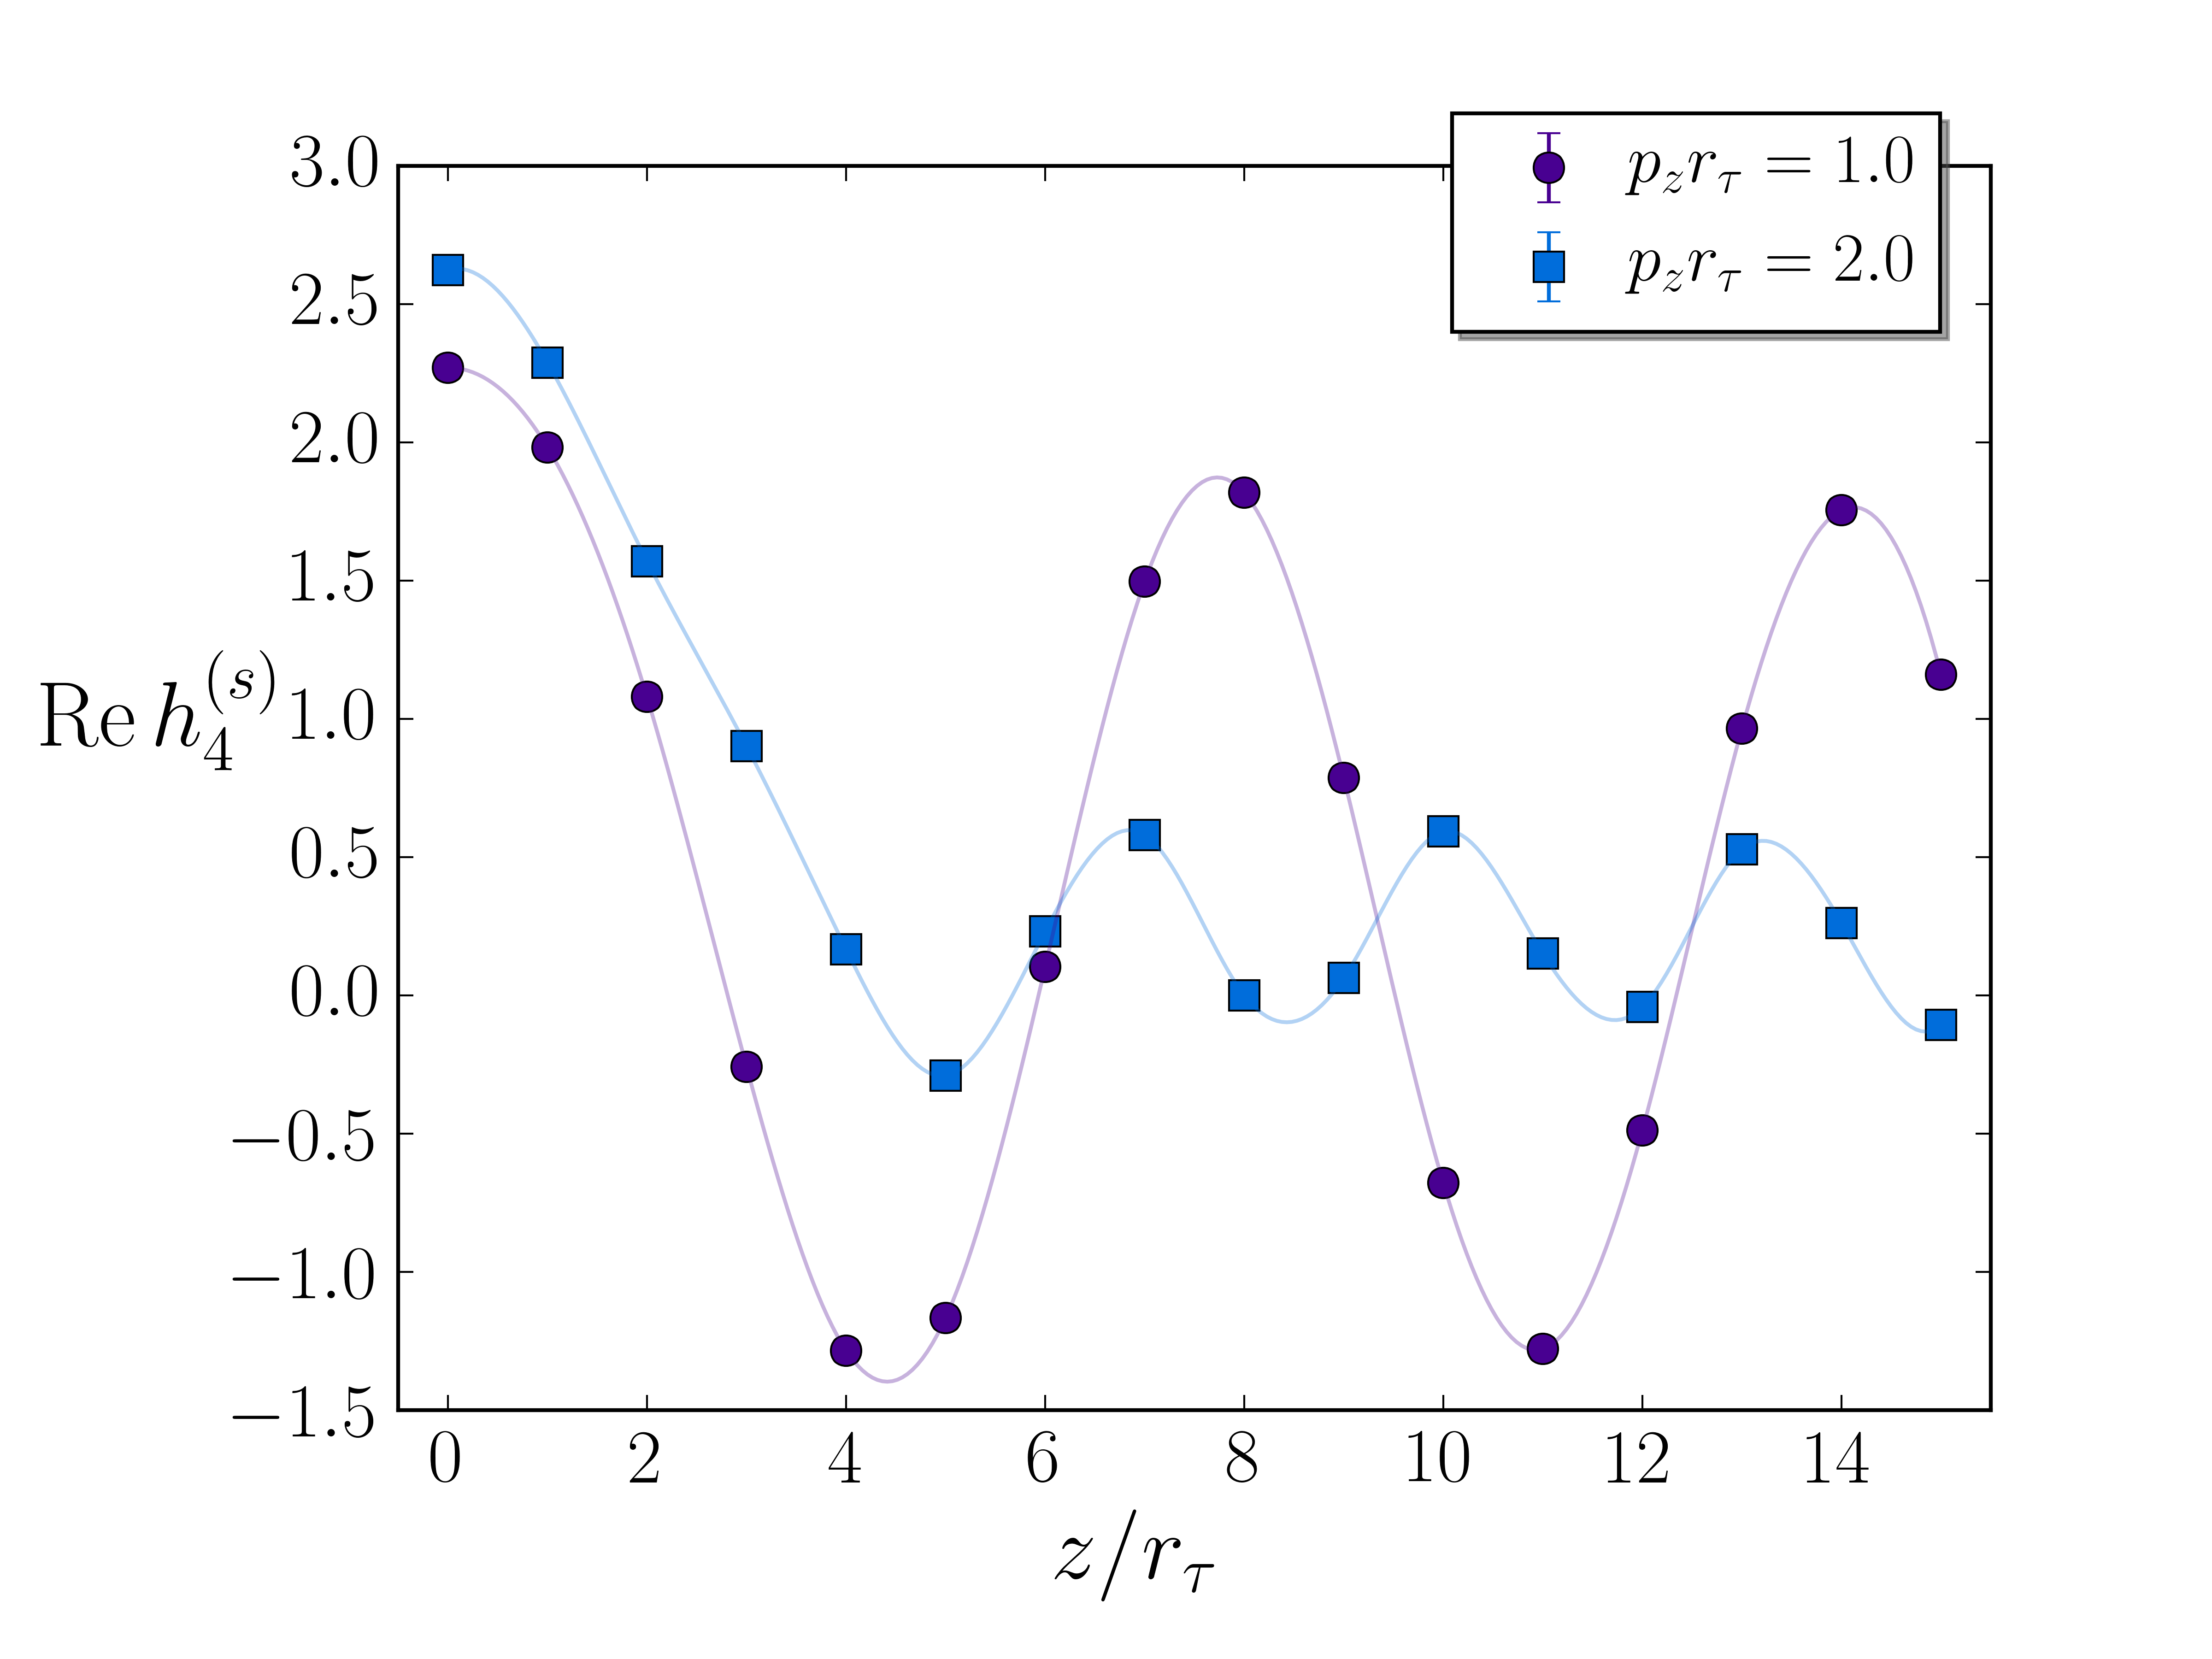
\includegraphics[width=0.4\textwidth,keepaspectratio]{images/hfn_re.png}\\
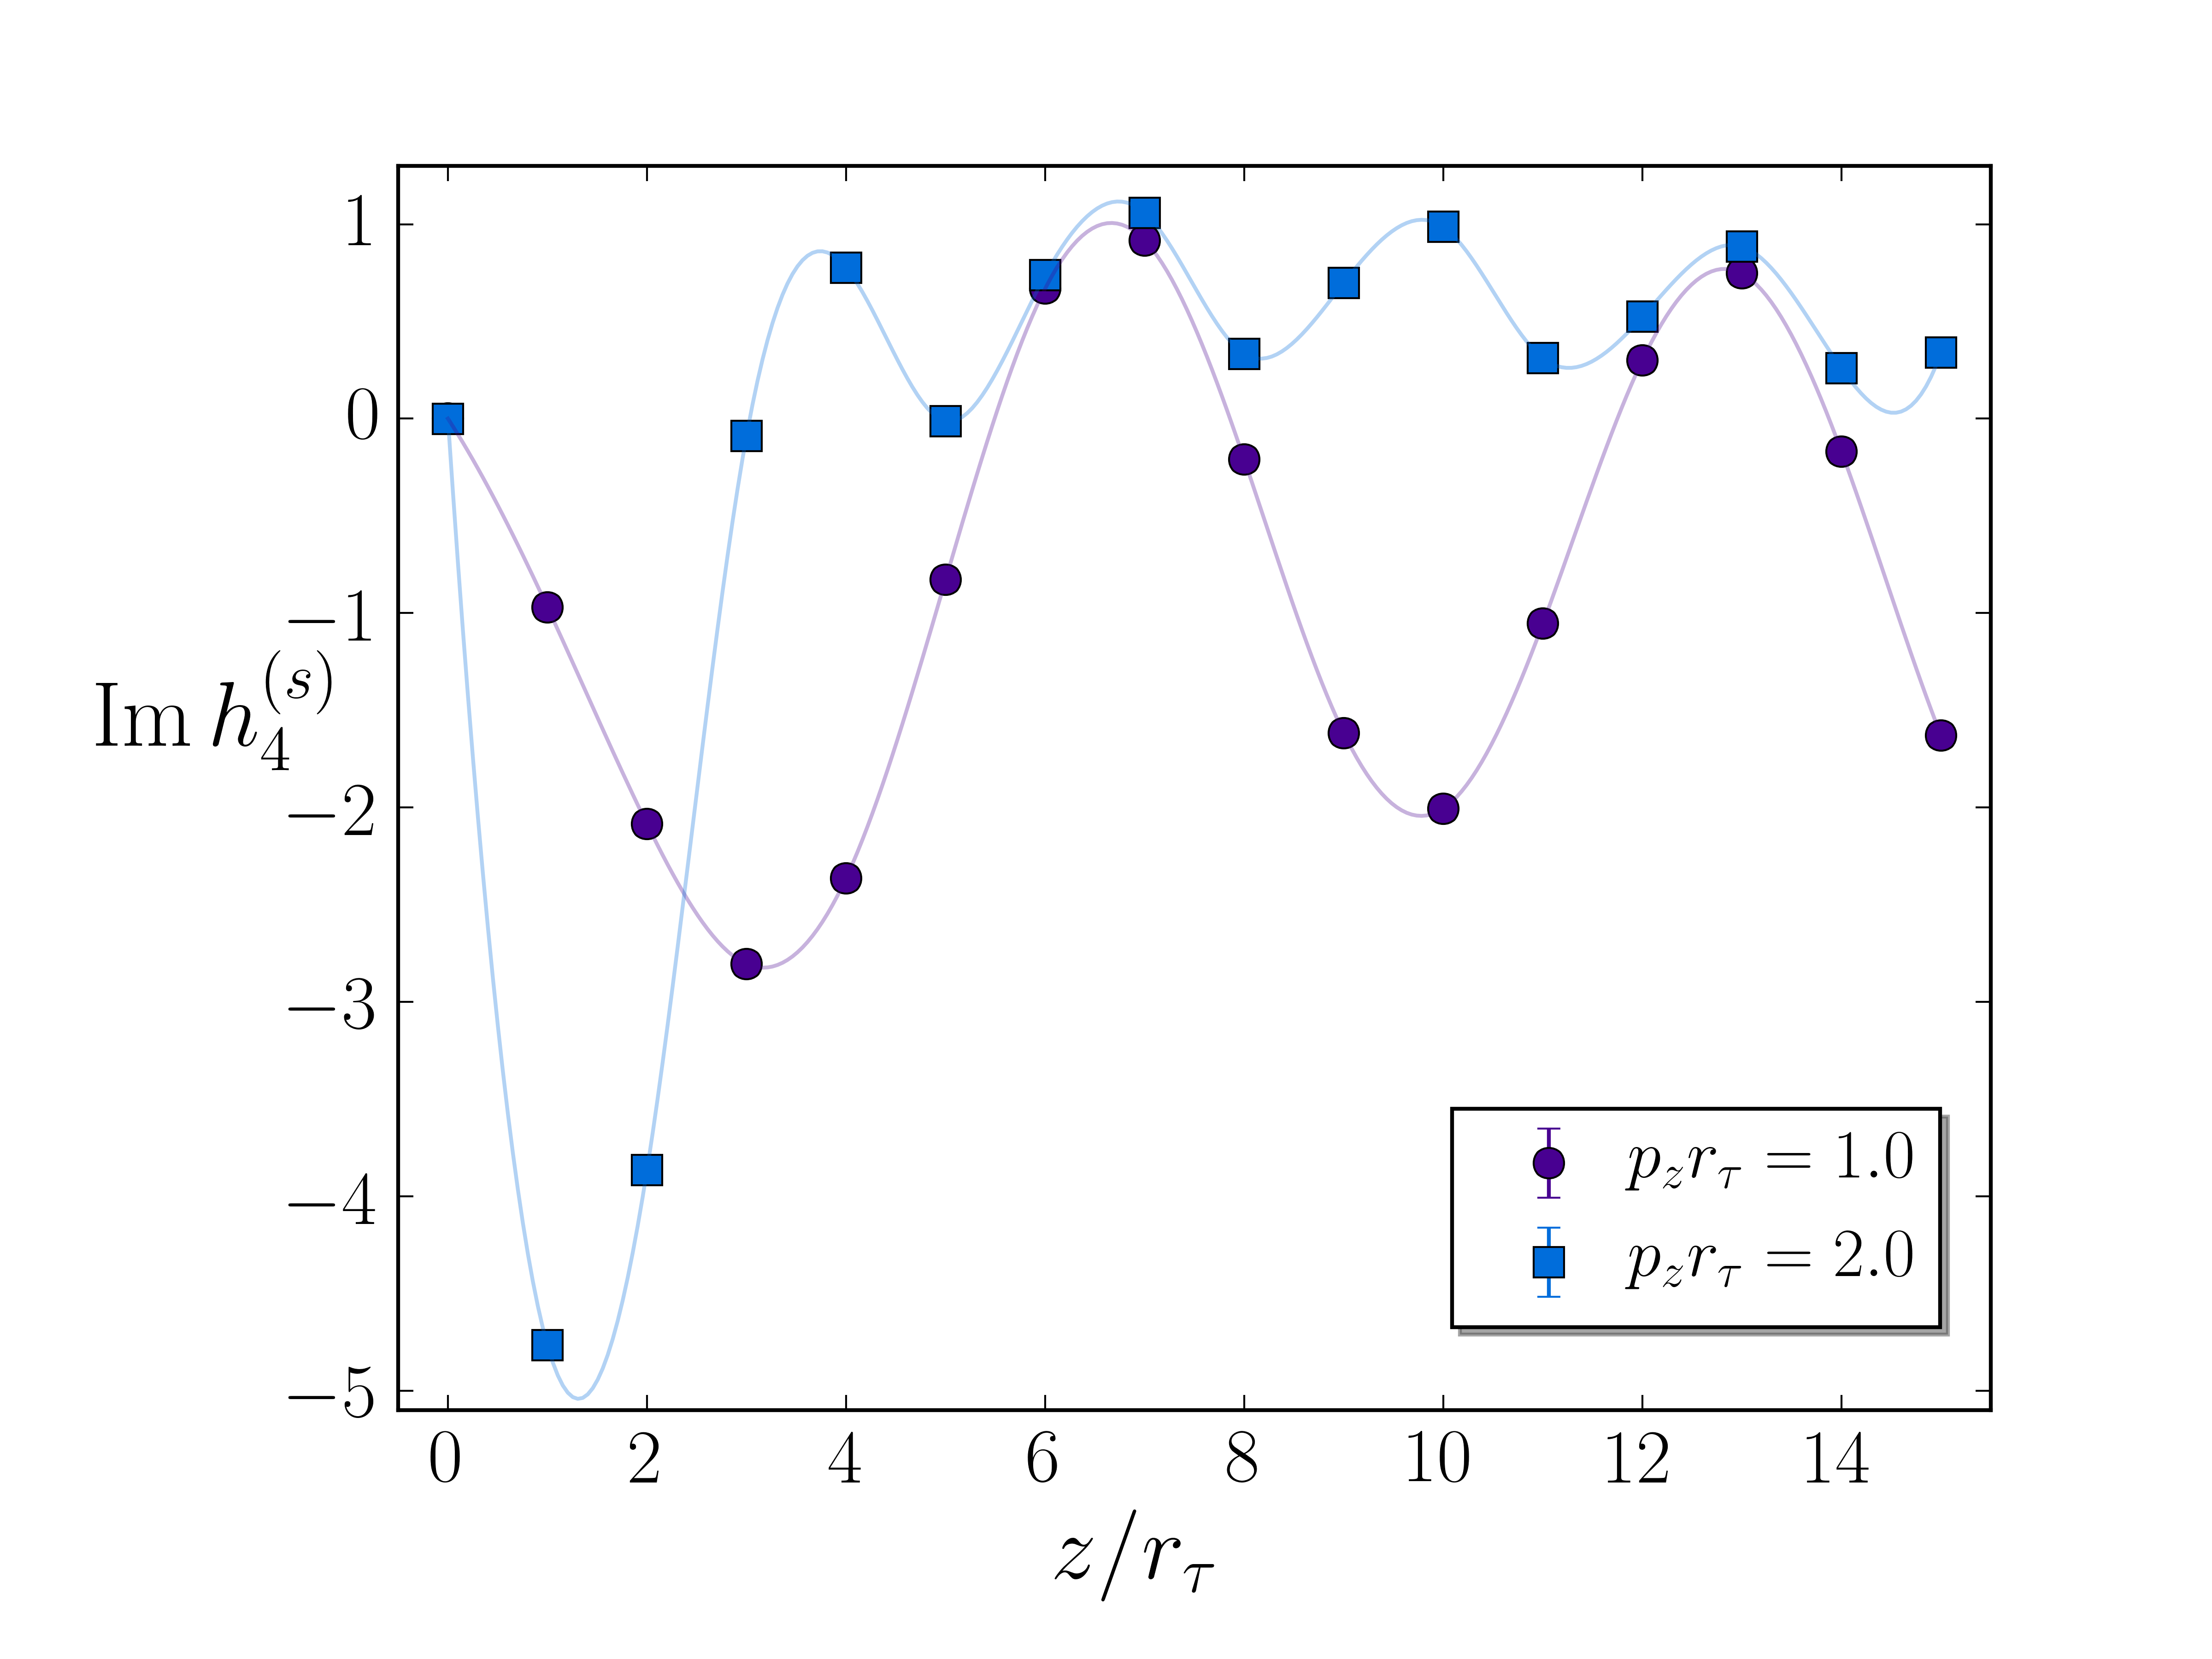
\includegraphics[width=0.4\textwidth,keepaspectratio]{images/hfn_im.png}
\end{figure}
